\documentclass[a4paper,12pt]{article}
\usepackage{graphicx}
\usepackage{hyperref}
\usepackage[titletoc,title]{appendix}
\usepackage{wrapfig}
\begin{document}
\title{Chomp
\subsubsection*{Requirements and Specification Document -- Group 6}\subsubsection*{Version 0.1}
}\maketitle

\renewcommand{\abstractname}{Project Abstract}
\begin{abstract}

Chomp is a web application that tracks what a person, group, or family eats, and gives nutritional advice, financial suggestions, sustainability ratings, and other meal and dietary statistical analysis.  Chomp provides a more digestable understanding of how our food affects us beyond a simple calorie counter.  By leveraging multiple informational APIs, a wealth of data can be generated from simple meal entries.  Customers use Chomp to gauge their daily, weekly, monthly, and quarterly progress toward their personal goals, and choose Chomp as their preffered tool because of its variety and wealth of information packed into a convenient and understandable form.  Plans for Chomp include adding a social support network of like-minded users to aid in users' feeling of and drive for success.  The anticipated revenue stream for Chomp will be in-app addvertisements that target a given user.\\
\\
Our github location is \url{http://github.com/hedekar/chomp} and the most recent version of this document is available there.
\end{abstract}
\newpage
\tableofcontents
\newpage
%%%%%%%%%%%%%%%%%%%%%%%%%%%%%%%%%%%%%%%%%%%%%%%%%%%
\section{Customers}
\subsection{Weight Loss}
This customer uses Chomp to keep a daily count of their calories and specific nutritional information to assist them in losing weight.  See \textbf{Appendix A.1} for the user persona of Boris Chetznekov for further info.
\subsection{Family Nutrition}
This customer uses Chomp to track how nutritious her family meals are and what deficiencies in the diet may need to be addressed.  She is also very concerned with meal cost.  See \textbf{Appendix A.2} for the user persona of Susan Montgomery for further info.
\subsection{Body Builder}
This customer uses Chomp to monitor his body's nutrition levels as he prepares for body building competitions.  He lives with two roommates who also work out, but not to the same level of competitiveness.  They all share groceries.  See \textbf{Appendix A.3} for the user persona of Chet Reist for further info.
%%%%%%%%%%%%%%%%%%%%%%%%%%%%%%%%%%%%%%%%%%%%%%%%%%%
\section{Competitive Analysis}
Many other meal-tracking services already exist.  Some have multiple million downloads and users.  The majority of these however are very specific in scope, with only calories being counted or with a focus on reporting all the nutritional numbers at once.  The large majority of these applications are targeting weight loss customers but not other users.\\
\\
Both web applications and mobile applications have been developed in this field.  Some specific competitors include: \begin{list}{•}{•}
\item \textbf{\href{http://www.noom.com}{Noom Coach -- noom.com} -- }A semi-free app that counts calories eaten and calories burned.  It then calculates and tracks weight of the user.  Includes 'coach' messages in a personalized manner.  The paid version allows for community sharing of progress and chatting amongst similar-goaled users as well as meal suggestions.  10-50million android downloads, 4.3 rating from 160,000+ reviews.  Its strengths are the personal coaching aspects and its very simple interface.
\item \textbf{\href{http://www.myfitnesspal.com}{MyFitnessPal -- myfitnesspal.com} -- }A full-featured free application and web app sponsored by UnderArmour.  Multiple nutrition reports are available for a user, though it is centred on calories, including a very complete meal item search list along with workout habits and daily activity settings.  This application is most closely related to our desired toolset, however the overall interface is very cumbersome to use on a daily basis.10-50million android downloads, 4.6 rating from 1.1milllion+ reviews.  Its strengths are the comprehensiveness of the information it gives while the user interface and the lack of group features are its downfalls.
\item \textbf{\href{http://www.lifesum.com}{Lifesum -- lifesum.com} -- }A semi-free app that heavily promotes the gold/paid upgrade.  Lifesum focuses primarily on meal suggestions with a substantial number of possible diet choices.  Meal suggestions come with full cooking instructions and basic (free) or complete (gold) nutritional information.  The recipe api used is from Recipies+ and their logo is used in the process.  The interface is very clean but with somewhat hidden and undiscoverable functionalities.  1-5million android downloads, 4.2 rating from 45,000 reviews.  Its strengths are the visually appealing interface and good meal suggestions, while its weaknesses include a difficult to understand interface and an incomplete feature set unless the upgrade is purchased.
\item \textbf{\href{http://www.fatsecret.com}{FatSecret -- fatsecret.com} -- }A very sleek and easy to use free meal and exercise diary.  The interface is extremely easy to use on a daily basis, includes weight tracking, a barcode scanner, and a community feed.  It is one of the few apps that editing mistake entries is immediately obvious, and readily gives nutritional breakdown for each food item.  10-50million android installs, 4.3 rating from 185,000+ reviews.  Its strengths are the ease of use and wealth of information, while its downfalls are a lack of summary reporting and a cold aesthetic.
\item \textbf{\href{http://www.myfooddiary.com}{My Food Diary -- myfooddiary.com} -- }A paid subscription website that charges \$9 per month for meal and excercise tracking.  It relies heavily on mainstream media advertisements for its customer base.  Includes a detailed body measures in its reports where a person can track waist, shoulders, etc... as well as nutritional breakdowns of a person's diet and any given food (fiber, iron, etc...).  There are customizable chart reporting and community features. The interface does look slightly clunky with poor web redered fonts but an update sneak peak via twitter shows a nicer interface.  User data is not known for this application, but LinkedIn lists them as having 1-10 employees.
\end{list}
It should be noted that despite heavy market saturation, the revenue stream will still exist for any application that can garner a reliable or substantial user base.  A large number of regular users is our target fiscal goal.\\
Furthermore, although many of these applications have strong features, none have the entire package of usability and full time-domain reporting.  None of the apps we reviewed featured a cost of meal tracker.  There is a space for Chomp in this market.
%%%%%%%%%%%%%%%%%%%%%%%%%%%%%%%%%%%%%%%%%%%%%%%%%%%
\section{User Stories}
%%%%%%%%% to include in each story: Name/Description, Actors/Personas, Precondition/trigger, Actions/Post Condition, Acceptance Criteria, Tests
\subsection{User Accounts}
\textbf{Personas involved:} All\\
\textbf{Description:} These stories are all united under the epic of editing and using both new and existing user accounts.  New users must first complete the Registration story.  Returning users must first complete the Login story.  After these stories, users may then complete the Account Setup and Logout stories.
\subsubsection{Registration}
\textbf{Precondition:} An unrecognized or not-logged in user visits our frontpage.\\
\textbf{Actions:} A user is greeted with an interface requesting to register.  Options for both Google and Facebook account linkage (via their account APIs) will be presented as well as a manual entry field for e-mail and password. \begin{list}{•}{•}
\item Google's API registration will request the user for their google e-mail and password.  After this is submitted, the
\item Facebook's API registration will request the user for their Facebook e-mail and password.  This will then re-direct to a facebook window that asks the user to agree for us to get certain 
\item Manual entry process will request first name, last name, username, and e-mail.  This will be followed up by sending the user's e-mail a confirmation message in which a unique activation link will be sent.  The process will end at a page instructing users to look for their e-mail link that will allow them to finish setting up their account.
\end{list}
After registration completion, the system will send the user directly to the Account Setup stage.\\
\textbf{Test/Postcondition:} A new account should be attempted to be created via google, facebook, as well as manually and the database should register all of the user's submitted information.  To check, developers can access the database directly to see the adition.
\subsubsection{Account Setup}
\textbf{Precondition:} Either the user's account has freshly been registered, or they have clicked on the 'Account Settings' button of their user profile.\\
\textbf{Actions:} If the account is already setup, the dialogue will present the setup items as an editable listing rather than sequential prompts.  A dialogue will ask the user about the following items\begin{list}{•}{•}
\item Number of users to track (along with their usernames if they're also Chomp users)
\item Birthdate (of primary user and each non-Chomp user)
\item Current weight (of primary user and each non-Chomp user)
\item Height (of primary user and each non-Chomp user)
\item Personal priority ranking (eg. sustainability, carbohydrate intake, finances, etc..)
\end{list}
Once all of this information is submitted, the user's account will be updated and the desired statistics will take priority in the nutrition and value tracking interface.  The user will see the saved account settings filled out with the option to re-edit them or to return to the home screen.\\
\textbf{Test/Postcondition:} To confirm that the information was saved to the user's account the simplest method is to check the database entry manually.  Once the entire user interface has be implemented, the changes of this process should be visible immediately on the user's homescreen.
\subsubsection{Login}
\textbf{Precondition:} A registered user is returning to the site without a login cookie in their browser.\\
\textbf{Actions:} At the centre of the screen the both username or e-mail field and password field will display for the user.  Once the fields are filled out, the user clicks the Login button.  If any error occurs, the user is notified of the problem (in a semi-specific manner that helps users without assisting intrusion attempts).  If no error occurs the user is taken to their Chomp homepage.\\
If an unregistered username or e-mail is entered, the registration process should begin for the user with a notice that the e-mail does not seem to be registered yet.\\
\textbf{Test/Postcondition:} An unregistered e-mail should be tried, at which time the user should be led to the registration story.  A registered account should be entered, first with an incorrect password, at which time an error message should appear, and then with a correct password, at which time the homescreen should appear.
\subsubsection{Logout}
\textbf{Precondition:} A user must be logged into their account.\\
\textbf{Actions:} By hovering over the user's name in the top-right corner of the screen a drop down menu will appear that includes the logout button.  The user then clicks this button and is greeted with the login screen.\\
\textbf{Test/Postcondition:} Follow the logout steps.  The login page should be reached.  Then attempt to visit a particular page of the user's profile.  This test should return an error.
%%%%%%%%%%%%%%%%%%%%%%%%%%%%%%%%%%%%%%%%%%%%%%%%%%%
\section{User Interface Requirements}
There are three major sections of our user interface that should be considered critical to the application's success.  Furthermore, we have ideas for expansion and additional feature that we will describe briefly in this section.
\subsection{Critical Interfaces}
\subsubsection{Meal Entry Dialogue}
This dialogue should allow entry for time of meal, contents of meal, and portion of meal.  Eventually, the ability to edit previous meals will also be added.
\subsubsection{Personal Nutrient \& Value Tracking}
This section of the homepage should give weekly, monthly, and yearly charts of the user's desired reporting figures and any additional abnormal trends our algorithm notices.
\subsubsection{Account Goal and Preference Adjustment}
This section is the user's administrative section over their entire account.  Here they can tweak what they want Chomp to help them with.
\subsection{Additional Interface Ideas}
These will be filled in in later iterations of this document.
\subsubsection{Suggested Meal Listing}
\subsubsection{Community Support Feed}
\subsubsection{Grocery Bill/List Tracking}
%%%%%%%%%%%%%%%%%%%%%%%%%%%%%%%%%%%%%%%%%%%%%%%%%%%
\newpage 
\begin{appendices}
\section{User Personas}
\subsection{Boris Chetznekov}
\begin{wrapfigure}{r}{0.5\textwidth}
  \begin{center}
	
\includegraphics[scale=0.3]{Boris.jpg}\\
  \end{center}
\end{wrapfigure}
\textbf{Age:} 58\\
\textbf{Weight:} 370lbs\\
\textbf{Occupation:} Office Manager for the city's traffic department\\
\textbf{Techy Rating:} 3.5 out of 5\\
\textbf{Goal:} To not die early.  After years of gross caloric intake his doctor has informed him of his impending death if his diet and weight doesn't change immediately.\\

\begin{large}
\textbf{\textit{"I guess I have to change my ways; stupid doctors.  Hopefully I can still drink a beer or vodka or two."}}
\end{large}\\\\
\textbf{Persona:} Boris grew up in a small Russian village for his first twenty five years before moving to Finland.  For years a diet of perogies, kielbasa, and beer have not been good to his cholesterol or his heart.  His wife has constantly asked him to eat a little less but Boris is very stubborn.\\
\\
Every Thursday the traffic office guys watch football at the pub, reminisce about when he was a fullback in Russia, and eat hot wings.  \textit{"There's no way I'm giving up hot wings and footy.  I might cut back on the wings, but I'm not giving them up, even if it kills me."}  Boris prefers the suicide flavour sauce that the pub makes in-house (the irony of that \textit{is} lost on him).\\
\\
His wife is fully in support of Boris's plan to lose weight and she'll cook whatever is needed for this to work -- or at least she'll try (she's not the best cook and often buys frozen dinners).  She does have a few recipes she loves to make (like borscht and kaalilaatikko/cabbage casserole), but often Boris and her share cooking duties, leading to many grilled-cheese dinners.  Rarely do they make salad.\\
\\
Boris is often the one in the office to sit at his desk and have people come to him.  It has been almost a decade since he had a shift in the field watching traffic flows or setting up car counters.  At home his reclining chair in front of the television is well-used.
\newpage
\subsection{Susan Montgomery}
\begin{wrapfigure}{r}{0.5\textwidth}
  \begin{center}
	
\includegraphics[scale=0.23]{Susan.jpg}
  \end{center}
\end{wrapfigure}
\textbf{Age:} 33\\
\textbf{Weight:} 143lbs\\
\textbf{Occupation:} Mother and part-time grocery clerk\\
\textbf{Techy Rating:} 2 out of 5\\
\textbf{Goal:} To ensure her two kids (as well as her and her husband) are eating healthy while also not going broke.\\
\\
\begin{large}
\textbf{\textit{"My family deserves the best foods we can afford.  I've heard spinach isn't as healthy as most think, and it's rather expensive."}}
\end{large}\\\\
\textbf{Persona:} Sue has a fussy five year-old son who really likes mac \& cheese, an eight year-old daughter who is a fairly adventurous eater but with a nut allergy, and an immature thirty-five year-old husband who doesn't like kale.  Susan's favourite treat is baked brie with apricot and crackers but she knows it goes straight to her hips.\\
\\
When the kids are in school Sue puts in four-hour shifts at the grocery store down the street to help with the family income.  Because of this she gets great discounts and often can snag products that are nearing expiration if she wants to.  Sometimes she wants to have that time free, but financially their family needs it.\\
\\
She loves watching the food TV shows but rarely has the time and wishes she had the same creativity of the chefs on TV.  Once she actually tried making ravioli from scratch, but ended up giving up half-way through because the kids were hungry.\\
\newpage
\subsection{Chet Reist}
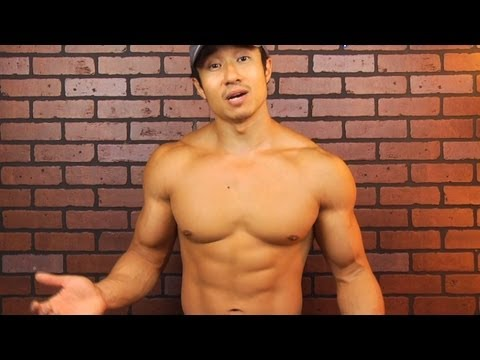
\includegraphics[scale=0.38]{Chet.jpg}\\
\textbf{Age:} 21\\
\textbf{Weight:} 170lbs\\
\textbf{Occupation:} Waiter and part-time supplement salesperson\\
\textbf{Techy Rating:} 4 out of 5\\
\textbf{Goal:} To win the next body building competition he enters and to keep track of how much of his food his roommates eat.\\
\begin{large}
\textbf{\textit{"I need protien, but I swear my roomates are taking my food whey when I'm not looking.  I ought to setup a camera to catch them."}}
\end{large}\\\\
\textbf{Persona:} Chet follows a daily routine as much as he can, but with his two jobs and shifting schedule, it's tough.  He tries to get in a protein shake and two bananas in the morning (whenever morning may be) before his daily workout.  Usually PowderPower has him scheduled in the afternoon for four hours before the evening shifts at the restaurant where he tries to grab dinner in the back between orders.  He's on closing shift right now, in hopes he can move to manager soon.\\
\\
He's getting sick of the food at the restaurant and is worried about its nutritional value.  When he gets home late he often has an easy though substantial meal (usually pasta) before surfing facebook and heading to bed.  He's not sure if that's terribly good for him.\\
\\
Both of his roommates often work out with Chet on his days off, but only Chet is actively working toward body building shows.  Because of this, his diet changes drastically in the month before a show and he follows whatever Jake at PowderPower tells him he should be eating.  Usually those meals get laid out for an entire week at a time but he has trouble sticking to the plan 100\%.
\end{appendices}
\end{document}